Um die grossen Datenmengen, die für ein robustes ML aus \ref{sec:DB} benötigt werden, liefern zu können, muss die Messung die teure menschliche Arbeitszeit drastisch reduzieren. Die Vorstudien in \ref{} erforderten rund 9 Stunden Arbeitszeit und hätten etwa 50 LWC-Tapes und 6 LWC-Denoth-Datenpunkte liefern können.

Ein grosser Vorteil des Tapes ist die feine örtliche Auflösung im zentel Millimeter Bereich in der Messregion von 20 x 20 mm. Um diese feine Auflösung zu nutzen, ist es spannend, Messungen durch die Höhe der Schneedecke durchzuführen.


Eine Möglichkeit besteht darin, dass der Feldforscher mit einer Bohrmaschine ein Loch in den Schnee bohrt. Dann kann das Messsystem in das Loch herabgelassen werden und kontinuierlich Messungen durchführen, während es abgesenkt wird.

Es ist auch möglich, dass das Messsystem über den Sommer an strategisch gewählten Orten aufgebaut wird und dann eingeschneit wird. Hier besteht die Schwierigkeit, an genügend 'ungetesteten' guten Schnee zu gelangen, um eine feine zeitliche Auflösung zu ermöglichen. Mit der vierten Iteration konnte gezeit werden, dass die Zeit nicht ein Problem darstellen muss.


Ein weiteres Konzept ist, dass das Messsystem von einem Helikopter aus abgeworfen wird. Durch die kinetische Energie schlägt das Messsystem dann durch die Schneedecke. In einer zweiten Phase wird das Tape an den Schnee angepresst und die Daten drahtlos an die Datenbank aus \ref{sec:DB} übermittelt.

Um den Anpressdruck seitlich ausüben zu können, funktioniert die Schwerkraft nicht mehr. Elastomere sind bei tiefen Temperaturen schwer einzuschätzen. Ein Elektromotor ist möglich, aber etwas mühsam mit der Batterie. Eine Blattfeder oder Kompressionsfeder sind vielversprechende Varianten. Ein pneumatisches System hat in der Wirkung vorteile, ist aber in der Umsetztung anspruchsvoll.

Das Tape kann auf eine Membran geklebt werden, die pneumatisch aufgeblasen wird und so an den Schnee angedrückt wird.

Um eine hohe Anpassbarkeit des steifen Tapes an den Schnee zu verbessern, kann das Tape in kleinere Stücke geschnitten werden. So kann sich der elastische Träger des Tapes effektiv an den Schnee anpassen.


\begin{figure}
    \centering
    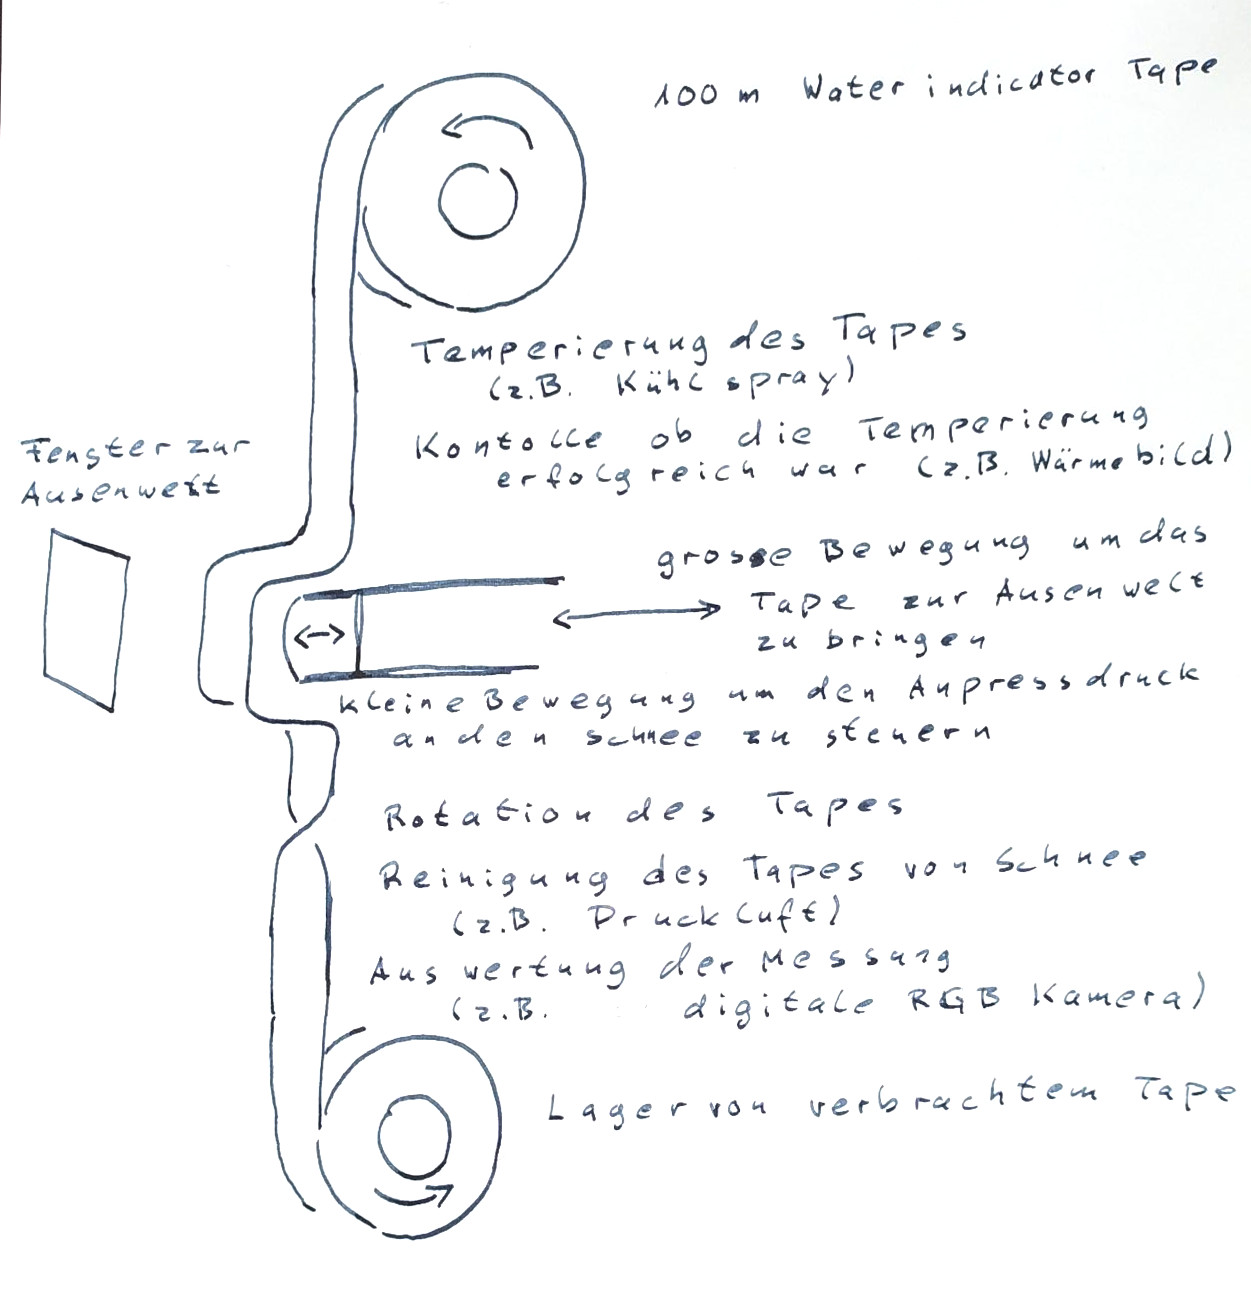
\includegraphics[width=0.8\textwidth]{Bilder/KonzeptAut.jpeg}
    \caption{Ablauf einer automatischen Messung}
    \label{fig:AutMess}
\end{figure}
